%%%%%%%%%%%%%%%%%%%%%%%%%%%%%%%%%%%%%%%%%
% Beamer Presentation
% LaTeX Template
% Version 1.0 (10/11/12)
%
% This template has been downloaded from:
% http://www.LaTeXTemplates.com
%
% License:
% CC BY-NC-SA 3.0 (http://creativecommons.org/licenses/by-nc-sa/3.0/)
%
%%%%%%%%%%%%%%%%%%%%%%%%%%%%%%%%%%%%%%%%%

%----------------------------------------------------------------------------------------
%    PACKAGES AND THEMES
%----------------------------------------------------------------------------------------

\documentclass[xcolor=dvipsnames,notes]{beamer}
\usepackage{pgfpages}
\usepackage{multicol}

\usepackage{color}
\usepackage{alltt}
\usepackage[T1]{fontenc}

% For graphics
\usepackage{tikz}
\usepackage{pgf}
\usepackage{xxcolor}
\usetikzlibrary{arrows,shadows,petri}
%%%%


\setbeameroption{show notes}
%\setbeameroption{show notes on second screen=right}

\mode<presentation> {

    \usetheme{Security}

}
\usepackage[utf8]{inputenc}
\usepackage[T1]{fontenc}
\usepackage{graphicx} % Allows including images
\usepackage{booktabs} % Allows the use of \toprule, \midrule and \bottomrule in tables

%----------------------------------------------------------------------------------------
%    TITLE PAGE
%----------------------------------------------------------------------------------------

\setbeamertemplate{footline}
{
    \leavevmode
    \hbox{
        \begin{beamercolorbox}[wd=.4\paperwidth,ht=2.25ex,dp=1ex,center]{author in head/foot}
            \usebeamerfont{author in head/foot}\insertshortauthor
        \end{beamercolorbox}
        \begin{beamercolorbox}[wd=.6\paperwidth,ht=2.25ex,dp=1ex,center]{title in head/foot}
            \usebeamerfont{title in head/foot}\insertshorttitle\hspace*{3em}
            \insertframenumber{} / \inserttotalframenumber\hspace*{1ex}
        \end{beamercolorbox}
    }
    \vskip0pt
}

\setbeamertemplate{navigation symbols}{}

\title[Administration des systèmes d'exploitation - Sécurité]{
        Administration des systèmes d'exploitation \\ Sécurité
}

\author{Etienne Papegnies} % Your name
\institute[UAPV] {
Université d'Avignon et des Pays de Vaucluse \\
    \medskip
    \textit{etienne.papegnies@univ-avignon.fr}
}
\date{2017} % Date, can be changed to a custom date

\begin{document}

%------------------------------------------------

\begin{frame}
\titlepage % Print the title page as the first slide
\end{frame}

%------------------------------------------------

\AtBeginSection[]
{
    \begin{frame}<beamer>
        \frametitle{Plan}
        \begin{multicols}{2}
            \tableofcontents[currentsection, subsectionstyle=hide]
        \end{multicols}
    \end{frame}
}



\AtBeginSubsection[]
{
   \begin{frame}
        \frametitle{Plan}
        \tableofcontents[
            currentsection,
            sectionstyle=show/hide,
            currentsubsection,
            subsectionstyle=show/shaded/hide
        ]
   \end{frame}
}




%------------------------------------------------------------------------------
%    PRESENTATION SLIDES
%------------------------------------------------------------------------------


%------------------------------------------------
\section{Surface d'Attaque}
%------------------------------------------------

\begin{frame}
\begin{columns}
\column{0.5\textwidth}
\begin{itemize}
    \item La surface d'attaque est un concept permettant d'évaluer le risque auquel est exposé un système informatique.
    \item Un ordinateur sans connexion Internet est dit "Air-Gapped"
\end{itemize}
\column{0.5\textwidth}
Ordinateur sans connexion Internet: quelle est la surface d'attaque?
\begin{figure}
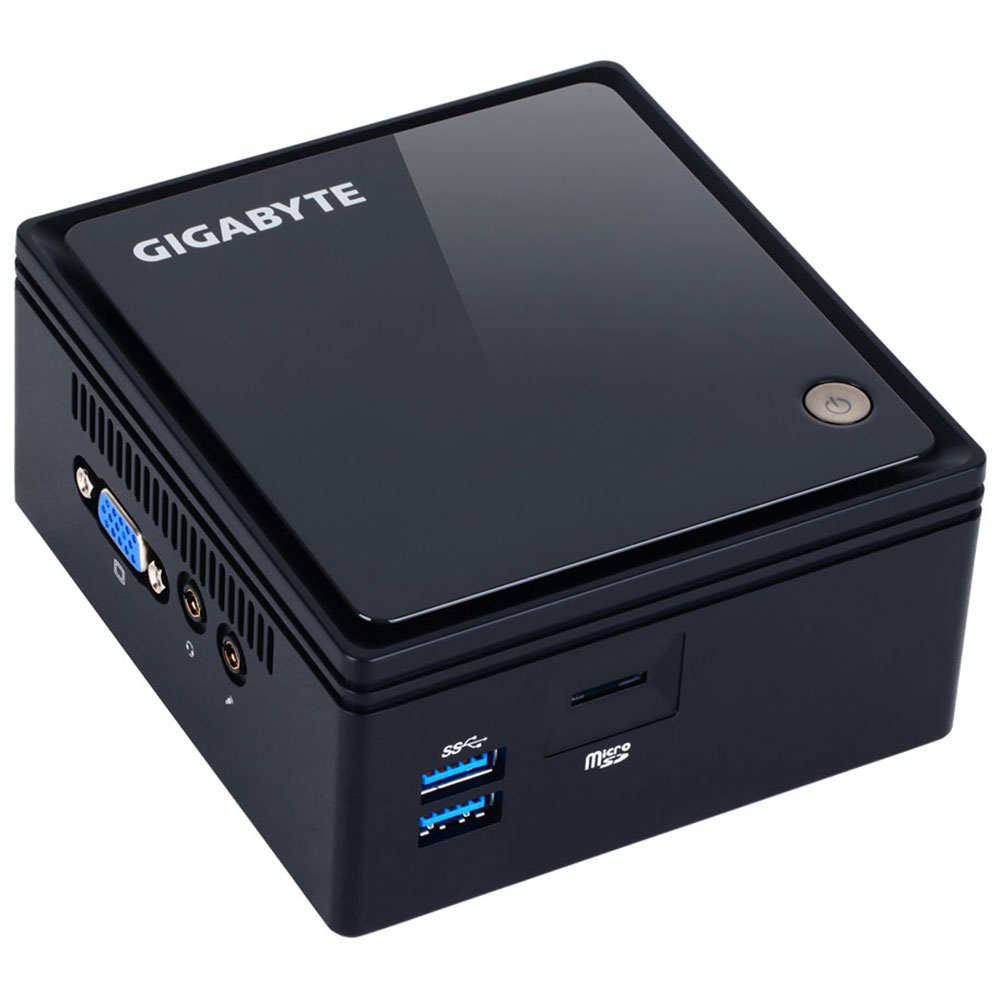
\includegraphics[scale=0.15]{res/brix}
\end{figure}
 
\end{columns}


\end{frame}
%------------------------------------------------

\begin{frame}
\begin{columns}
\column{0.5\textwidth}
\begin{itemize}
    \item La surface d'attaque est un concept permettant d'évaluer le risque auquel est exposé un système informatique.
    \item Un ordinateur sans connexion Internet est dit "Air-Gapped"
\end{itemize}
\column{0.5\textwidth}
Ordinateur sans connexion Internet: quelle est la surface d'attaque?
\begin{figure}
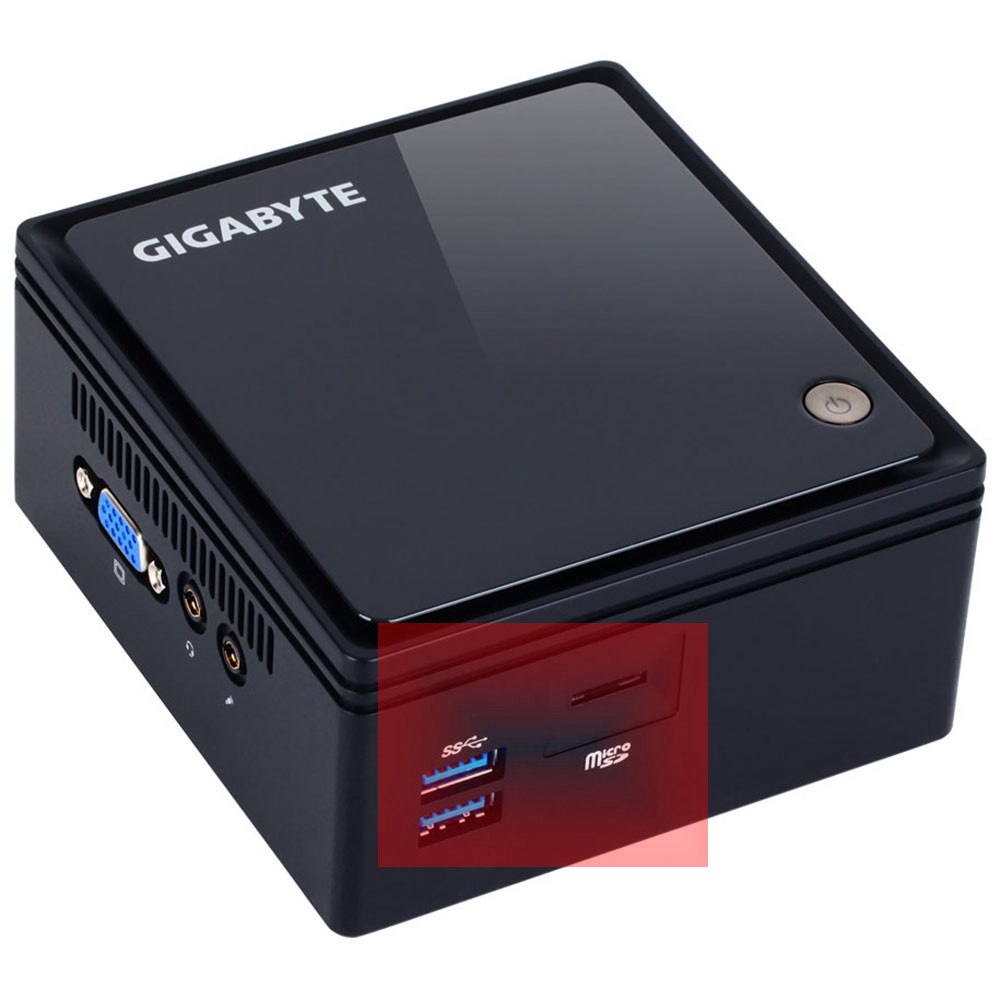
\includegraphics[scale=0.15]{res/brix2}
\end{figure}
Les ports USB.
\end{columns}


\end{frame}
%------------------------------------------------

\begin{frame}

L'USB c'est cool:
\begin{itemize}
    \item On branche une clef USB -> ça marche !
    \item On branche un clavier USB -> ça marche !
    \item Est-ce que une clef USB peut prétendre être un clavier ?
    \begin{itemize}
        \item Ouaip.
    \end{itemize}
\end{itemize}

\begin{figure}
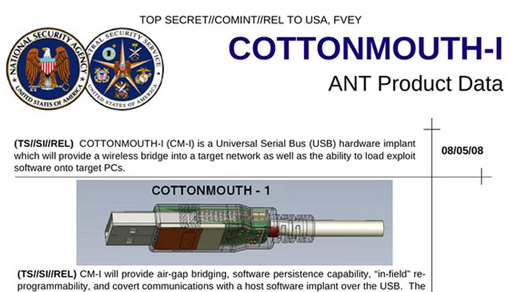
\includegraphics[scale=0.55]{res/badusb}
\end{figure}


\end{frame}

%------------------------------------------------

\begin{frame}
\begin{center}
Serveur connecté à internet, sans services.

\begin{itemize}
    \item Les ports Physiques (USB etc)
    \item Le driver réseau
    \item La fonction de routage du Kernel
\end{itemize}

+ serveur SSH.

\begin{itemize}
    \item Les ports Physiques (USB etc)
    \item Le driver réseau
    \item La fonction de routage du Kernel
    \item Le serveur SSH
\end{itemize}
\end{center}

\end{frame}



%------------------------------------------------
\begin{frame}

Station de travail sous Windows avec un antivirus connectée à internet, avec un employé qui consulte Facebook
\begin{itemize}
    \item Les ports Physiques (USB etc)
    \item Le driver réseau
    \item La fonction de routage du Kernel
    \item L'antivirus
    \item Le navigateur web
\end{itemize}

\end{frame}



%------------------------------------------------


\begin{frame}

Pour analyser la surface d'attaque, vous devez:
\begin{itemize}
    \item Noter tous les flux de données extérieures dans votre SI
    \item Recenser tout le matériel soumis à ces flux de données
    \item Recenser toute la couche logicielle soumis à ces flux de données
\end{itemize}

\end{frame}







%------------------------------------------------
\section{Hashing}
%------------------------------------------------

\subsection{Hash Function}

\begin{frame}


Fonction qui:
\begin{itemize}
    \item prends en entrée des données de taille arbitraire
    \item fait correspondre une sortie de taille fixe
    \item est déterministe
\end{itemize}

\begin{center}
\begin{minipage}[c]{0.7\linewidth}
% Style definition file generated by highlight 3.18, http://www.andre-simon.de/ 

% Highlighting theme: Kwrite Editor 

\newcommand{\hlstd}[1]{\textcolor[rgb]{0,0,0}{#1}}
\newcommand{\hlnum}[1]{\textcolor[rgb]{0.69,0.49,0}{#1}}
\newcommand{\hlesc}[1]{\textcolor[rgb]{1,0,1}{#1}}
\newcommand{\hlstr}[1]{\textcolor[rgb]{0.75,0.01,0.01}{#1}}
\newcommand{\hlpps}[1]{\textcolor[rgb]{0.51,0.51,0}{#1}}
\newcommand{\hlslc}[1]{\textcolor[rgb]{0.51,0.51,0.51}{\it{#1}}}
\newcommand{\hlcom}[1]{\textcolor[rgb]{0.51,0.51,0.51}{\it{#1}}}
\newcommand{\hlppc}[1]{\textcolor[rgb]{0,0.51,0}{#1}}
\newcommand{\hlopt}[1]{\textcolor[rgb]{0,0,0}{#1}}
\newcommand{\hlipl}[1]{\textcolor[rgb]{0,0.34,0.68}{#1}}
\newcommand{\hllin}[1]{\textcolor[rgb]{0.33,0.33,0.33}{#1}}
\newcommand{\hlkwa}[1]{\textcolor[rgb]{0,0,0}{\bf{#1}}}
\newcommand{\hlkwb}[1]{\textcolor[rgb]{0,0.34,0.68}{#1}}
\newcommand{\hlkwc}[1]{\textcolor[rgb]{0,0,0}{\bf{#1}}}
\newcommand{\hlkwd}[1]{\textcolor[rgb]{0,0,0.51}{#1}}
\definecolor{bgcolor}{rgb}{0.88,0.92,0.93}


\noindent
\ttfamily
\hlstd{}\hlslc{\#!\ /usr/bin/python\ {-}u}\hspace*{\fill}\\
\hlstd{}\hspace*{\fill}\\
\hlkwa{def\ }\hlstd{}\hlkwd{hash\textunderscore function}\hlstd{}\hlopt{(}\hlstd{text}\hlopt{):}\hspace*{\fill}\\
\hlstd{}\hlstd{\ \ \ \ }\hlstd{out\ }\hlopt{=\ }\hlstd{}\hlnum{0}\hspace*{\fill}\\
\hlstd{}\hlstd{\ \ \ \ }\hlstd{}\hlkwa{for\ }\hlstd{c\ }\hlkwa{in\ }\hlstd{text}\hlopt{:}\hspace*{\fill}\\
\hlstd{}\hlstd{\ \ \ \ \ \ \ \ }\hlstd{out\ }\hlopt{+=\ }\hlstd{}\hlkwb{ord}\hlstd{}\hlopt{(}\hlstd{c}\hlopt{)}\hspace*{\fill}\\
\hlstd{}\hlstd{\ \ \ \ }\hlstd{}\hlkwa{return\ }\hlstd{out\ \%\ }\hlnum{100}\hspace*{\fill}\\
\hlstd{}\hspace*{\fill}\\
\hlkwa{print\ }\hlstd{}\hlkwd{hash\textunderscore function}\hlstd{}\hlopt{(}\hlstd{}\hlstr{"hello"}\hlstd{}\hlopt{)}\hlstd{\ \ \ \ }\hlopt{}\hlstd{}\hlslc{\#\ {-}$>$\ 32}\hspace*{\fill}\\
\hlstd{}\hlkwa{print\ }\hlstd{}\hlkwd{hash\textunderscore function}\hlstd{}\hlopt{(}\hlstd{}\hlstr{"world"}\hlstd{}\hlopt{)}\hlstd{\ \ \ \ }\hlopt{}\hlstd{}\hlslc{\#\ {-}$>$\ 52}\hspace*{\fill}\\
\hlstd{}\hlkwa{print\ }\hlstd{}\hlkwd{hash\textunderscore function}\hlstd{}\hlopt{(}\hlstd{}\hlstr{"!"}\hlstd{}\hlopt{)}\hlstd{\ \ \ \ \ \ \ \ }\hlopt{}\hlstd{}\hlslc{\#\ {-}$>$\ 33}\hlstd{}\hspace*{\fill}\\
\mbox{}
\normalfont
\normalsize

\end{minipage}
\end{center}

\end{frame}

%------------------------------------------------




\subsection{Cryptographic Hash Function}
\begin{frame}
\frametitle{Introduction}
\begin{itemize}
    \item Une fonction de hachage avec les propriétés:
    \begin{itemize}
        \item Est rapide à calculer quelque soit la taille de l'entrée
        \item A un espace de sortie suffisamment large
        \item Un petit changement dans l'entrée provoque une cascade de changements en sortie
        \item En utilisant la sortie, il est difficile de re-créer l'entrée
        \item Si on a l'entrée et la sortie, il est difficile de trouver une autre entrée avec la même sortie
    \end{itemize}
\end{itemize}
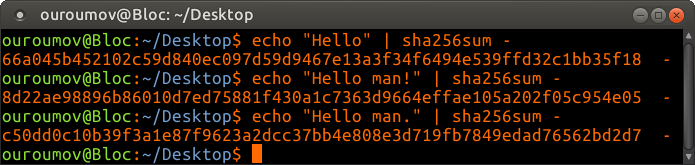
\includegraphics[scale=.5]{res/sha256sum}
\end{frame}


%------------------------------------------------


\subsection{Password Hash Function}
\begin{frame}
Une fonction de hachage pour mots de passe doit:
\begin{itemize}
    \item Avoir les propriétés d'une fonction de hachage cryptographique
    \item Utiliser un Sel concaténé avec le mot de passe
    \item Être configurable pour pouvoir consommer:
    \begin{itemize}
        \item Une quantité de mémoire arbitraire
        \item Un nombre de cycles CPU arbitraire
    \end{itemize}
\end{itemize}

\begin{center}
BCrypt Hash Function, cost level 10
\end{center}
\resizebox{\textwidth}{!}{%
    \begin{tabular}{ c | c | c }
    Password & Salt & Hash \\ \hline
    \texttt{Passw0rd} & \textcolor{blue}{\texttt{Q/AzxLshsyaAqptlgni74u}} & \texttt{\$2a\$10\$}\textcolor{blue}{\texttt{Q/AzxLshsyaAqptlgni74u}}\textcolor{green}{\texttt{N5WQrGCW176CPbPSVqrt/pUNS7HW9tu}} \\ \hline
    \texttt{lolwhat}  & \textcolor{blue}{\texttt{7JYaQZA9w/PGfv4C0ab92O}} & \texttt{\$2a\$10\$}\textcolor{blue}{\texttt{7JYaQZA9w/PGfv4C0ab92O}}\textcolor{green}{\texttt{qmH.YFrQmucp1wqRfUEd3KHI/ty6dHm}} \\ \hline
    \texttt{lolwhat}  & \textcolor{blue}{\texttt{02h4313J6Qgs/3daZ/iaze}} & \texttt{\$2a\$10\$}\textcolor{blue}{\texttt{02h4313J6Qgs/3daZ/iaze}}\textcolor{green}{\texttt{9RJR3EIblB6HZRX8zAWuP3TNKSY1zDu}} \\ \hline
    \end{tabular}
}

\end{frame}

%------------------------------------------------



%------------------------------------------------
\section{Chiffrement Asymétrique}
%------------------------------------------------

\begin{frame}
    \frametitle{Introduction}
    \begin{itemize}
        \item Méthode de chiffrement a deux clefs
        \item Ce qui est chiffré avec une clef ne peut être déchiffré que par l'autre
    \end{itemize}
    \begin{center}
        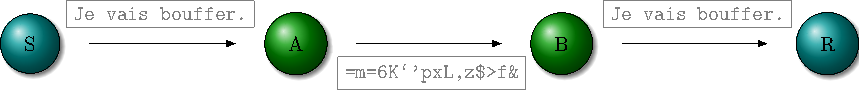
\includegraphics[scale=0.7]{res-src/asym_crypto}
        \vspace{4em}
        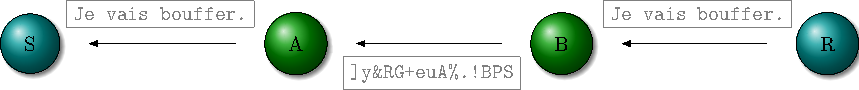
\includegraphics[scale=0.7]{res-src/asym_cryptor}
    \end{center}
\end{frame}

%------------------------------------------------

\begin{frame}
\frametitle{Communication chiffrée de Bob vers Alice}
    \begin{center}
        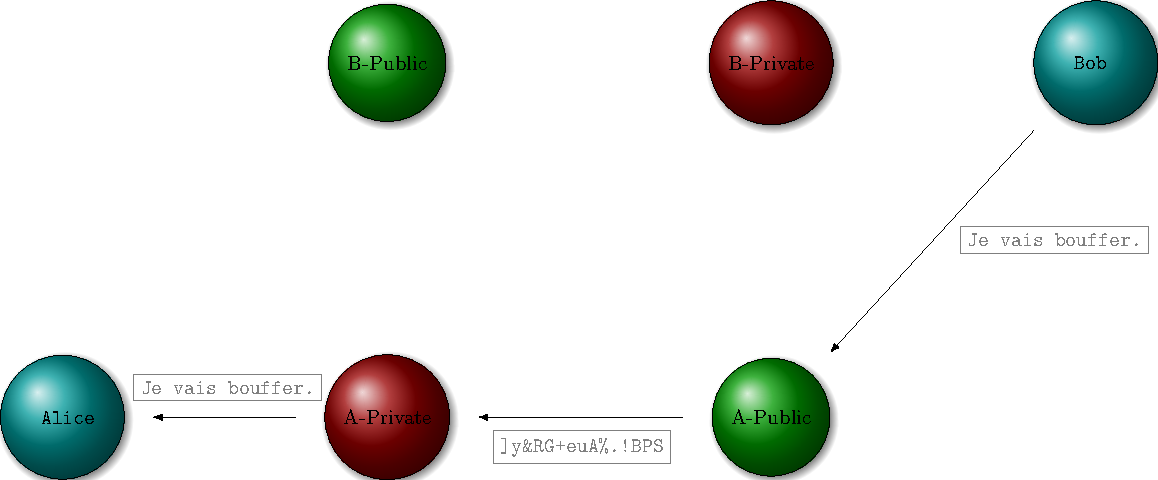
\includegraphics[scale=0.55]{res-src/asym_crypto_com}
    \end{center}
    \begin{itemize}
        \item Bob est sûr que Alice est la seule à pouvoir lire le message
        \item Alice ne sait pas qui est l'auteur du message
    \end{itemize}
\end{frame}

%------------------------------------------------

\begin{frame}
\frametitle{Réponse en clair de Alice avec Signature du message}
    \begin{center}
        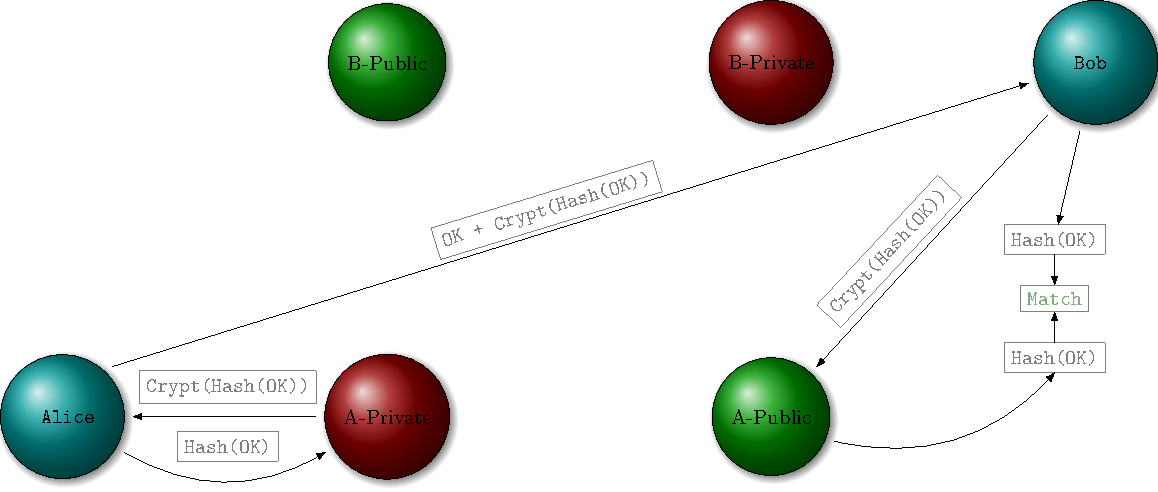
\includegraphics[scale=0.55]{res-src/asym_crypto_sign}
    \end{center}
    \begin{itemize}
        \item Alice envoie message en clair + hash chiffré par sa clef privée
        \item Bob déchiffre le hash de Alice, et calcule le hash de son côté
    \end{itemize}
\end{frame}



%------------------------------------------------
\section{MITM \& HTTPS}
%------------------------------------------------

\subsection{MITM}
\begin{frame}
\begin{center}
Le type au millieu.\\

\includegraphics[scale=0.80]{res/mitm}\\
Quelqu'un en position de MITM peut:
\begin{itemize}
    \item Intercepter le traffic
    \item Modifier le traffic
\end{itemize}
\end{center}
\end{frame}



%------------------------------------------------
\subsection{HTTP}
\begin{frame}
\frametitle{HTTP}

\begin{itemize}
    \item HTTP est ni authentifié, ni encrypté.
    \item Certains acteurs peux scrupuleux utilisent ça pour lancer des DDoS massifs
\end{itemize}
\begin{center}
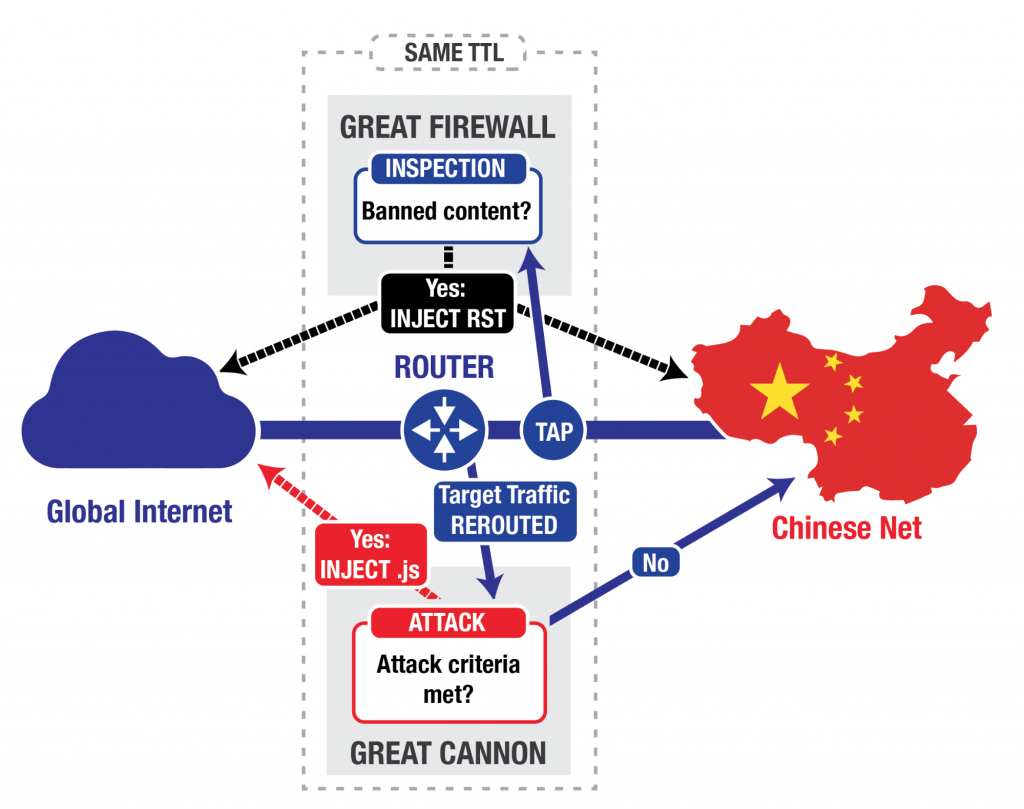
\includegraphics[scale=0.20]{res/great_cannon}
\end{center}
\end{frame}

\note{

    \href{https://arstechnica.com/security/2015/04/meet-great-cannon-the-man-in-the-middle-weapon-china-used-on-github/}{\beamergotobutton{Ars Technica's article on China's "Great Cannon"}}

}


%------------------------------------------------
\subsection{HTTPS}
\begin{frame}
    \frametitle{HTTPS}
    \begin{itemize}
        \item La version "sûre" de HTTP
        \item À la fois encrypté et authentifié
        \item Meilleur système actuel pour protéger le traffic, mais loin d'être idéal 
        \item Depuis l'apparition de "Let's Encrypt", il n'y a plus d'excuse pour ne pas protéger le traffic de son site
    \end{itemize}
\end{frame}

\begin{frame}
    \frametitle{HTTPS: implémentation}
    \begin{itemize}
        \item Crypto Asymétrique pour l'établissement de la connexion
        \item Utilisation de certificats contenant des clefs publiques
        \item Crypto symétrique pour le gros du traffic
    \end{itemize}
\end{frame}

\note{

    \href{http://www.moserware.com/2009/06/first-few-milliseconds-of-https.html}{\beamergotobutton{A nice technical analysis of what happens at the begining of an HTTPS connection}}
    \begin{center}
    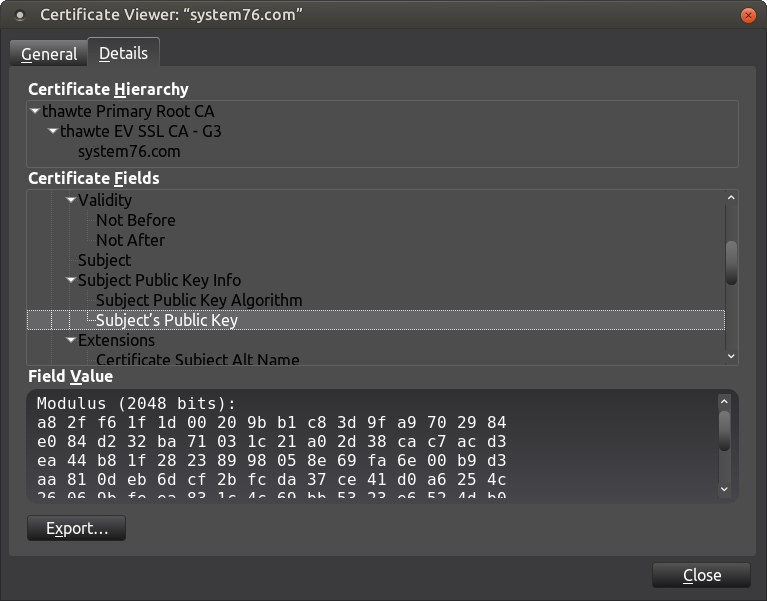
\includegraphics[scale=0.30]{res/https_cert}
    \end{center}
}

\begin{frame}
    \frametitle{HTTPS: Problèmes}
    \begin{itemize}
        \item Basé sur une chaîne de confiance
        \begin{itemize}
            \item Grand nombre de CAs "root"
            \item Contrôle d'un CA 'root' permet de MITM le traffic
            \item Certains CAs ne sont pas dignes de confiance
        \end{itemize}
        \item Approche souvent trop tolérante car
        \begin{itemize}
            \item Les entreprises ont de l'inertie
            \item Sécurité moyenne > Pas de sécurité
        \end{itemize}
    \end{itemize}
\end{frame}
















%------------------------------------------------
\section{Vulnérabilités}
%------------------------------------------------

\begin{frame}
\frametitle{Types de vulnérabilités}

Il existe de nombreux types de vulnérabilités, mais il est pratique de les lister par type d'impact possibles:
\begin{itemize}
 \item Denial Of Service % Bash ForkBomb
 \item Information Leakage % Heartbleed
 \item Man In The Middle % Lenovo Superfish
 \item Privilege Escalation % Rowhammer
 \item Remote Code Execution % Shellshock

\end{itemize}

\end{frame}

\subsection{Denial Of Service}
\begin{frame}
\frametitle{Exemple: Fork Bomb}

\begin{center}

\includegraphics[scale=0.55]{res/bash_fork}
\end{center}

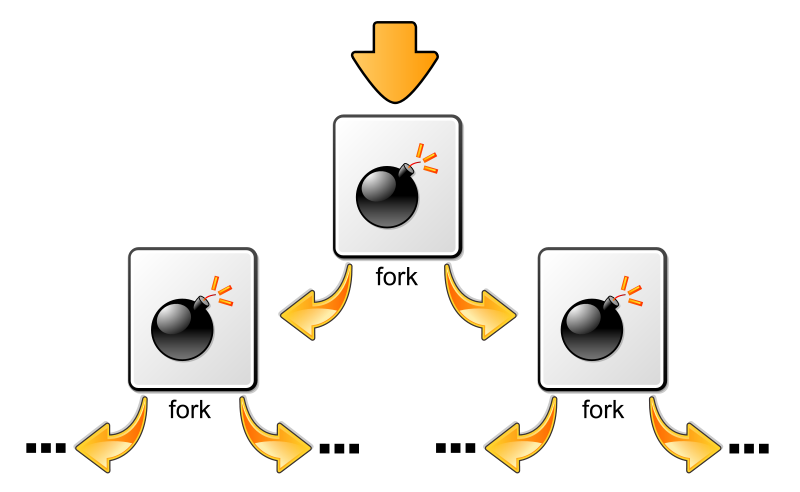
\includegraphics[scale=0.24]{res/fork_bomb}
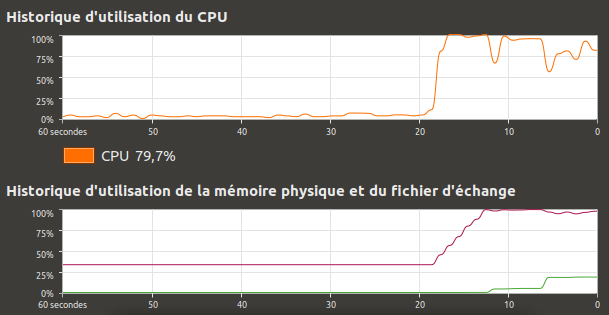
\includegraphics[scale=0.24]{res/DoS}

\end{frame}




\subsection{Information Leakage}
\begin{frame}
\frametitle{Exemple: Heartbleed}

\begin{center}
    Heartbleed\\
    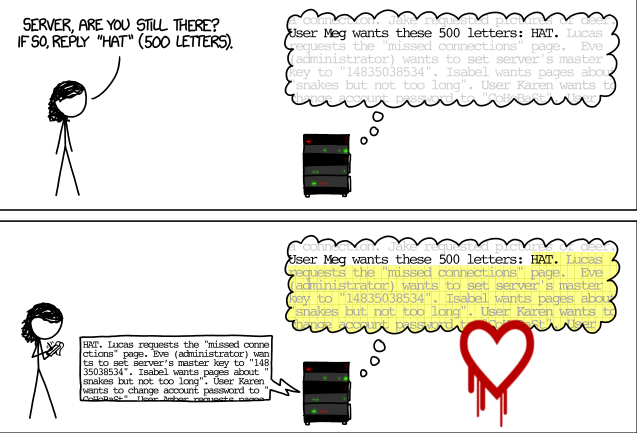
\includegraphics[scale=0.44]{res/heartbleed_explanation}
\end{center}


\end{frame}


\note{

     \href{https://arstechnica.com/security/2014/04/critical-crypto-bug-in-openssl-opens-two-thirds-of-the-web-to-eavesdropping/}{\beamergotobutton{
        Heartbleed: Ars Technica Article
    }}\\

    \href{https://xkcd.com/1354/}{\beamergotobutton{
        Heartbleed: xkcd explanation
    }}

}

\subsection{Man In The Middle}
\begin{frame}
\frametitle{Exemple: Superfish}

\begin{center}
    Lenovo's Massive Fuckup\\
    \vspace{3em}
    
\includegraphics[scale=0.24]{res/superfish}
\end{center}


\end{frame}

\note{

    \href{https://arstechnica.com/security/2015/02/lenovo-pcs-ship-with-man-in-the-middle-adware-that-breaks-https-connections/}{\beamergotobutton{
        Why I don't like Lenovo
    }}

}






\subsection{Privilege Escalation}
\begin{frame}
\frametitle{Exemple: Rowhammer}

\begin{center}
    Physical attack on DRAM memory\\
    \vspace{2em}
    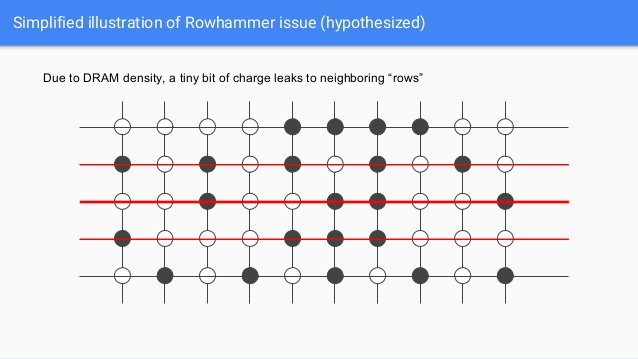
\includegraphics[scale=0.24]{res/rowhammer}
\end{center}
\begin{itemize}
    \item En changeant les valeurs d'une page de mémoire répétitivement, il est possible de faire changer la valeur de Bits dans la page d'à côté.
    \item Cela peut permettre à un programme tournant avec des privilèges utilisateurs d'obtenir les privilèges de root.
\end{itemize}
\end{frame}

\note{

    \href{https://googleprojectzero.blogspot.fr/2015/03/exploiting-dram-rowhammer-bug-to-gain.html}{\beamergotobutton{
        Project Zero writeup on Rowhammer
    }}

}




\subsection{Remote Code Execution}
\begin{frame}
\frametitle{Exemple: Shellshock}

\begin{center}
    24 Septembre 2014\\
    Une des pires vulnérabilités de tout les temps.\\
    \vspace{2em}
    
\includegraphics[scale=0.54]{res/shellshock}
    \begin{itemize}
        \item Permet d'exécuter du code arbitraire sur des serveurs web
        \item Dans les jours suivant l'annonce, un scan automatique massif d'internet était en cours pour compromettre des serveurs
    \end{itemize}
\end{center}
\end{frame}



\note{
    \href{https://arstechnica.com/security/2014/09/bug-in-bash-shell-creates-big-security-hole-on-anything-with-nix-in-it/}{\beamergotobutton{
        Ars Technica's article on Shellshock
    }}


}





%------------------------------------------------
\section{Veille Technologique}
%------------------------------------------------

\begin{frame}
\frametitle{Veille Technologique}

\begin{center}
Si vous êtes responsable de la sécurité, il faut surveiller l'actualité.\\
\vspace{2em}

\includegraphics[scale=0.44]{res/cert}

\begin{itemize}
    \item Surveillez les sources d'informations
    \begin{itemize}
        \item CERT
        \item Ars Technica
        \item Slashdot
        \item Podcasts de sécurité ( twit.tv/sn )
    \end{itemize}
    \item Utilisez l'analyse de votre surface d'attaque pour poser des alertes
    \begin{itemize}
        \item Sur le matériel que vous utilisez
        \item Sur les logiciels que vous utilisez
    \end{itemize}
\end{itemize}


\end{center}




\end{frame}

\note{


    \href{https://www.us-cert.gov/ncas/alerts}{\beamergotobutton{
        US-CERT
    }} \\
    \href{http://www.cert.ssi.gouv.fr/}{\beamergotobutton{
        FR-CERT
    }} \\
    \href{https://slashdot.org/}{\beamergotobutton{
        Slashdot
    }} \\
    \href{https://arstechnica.com/security/}{\beamergotobutton{
        Ars Technica
    }} \\
    \href{https://news.ycombinator.com/}{\beamergotobutton{
        Hackernews
    }} \\
    \href{https://www.twit.tv/shows/security-now}{\beamergotobutton{
        Weekly "Security Now" podcast by Steve Gibson
    }} \\
    \href{https://threatpost.com/}{\beamergotobutton{
        Threatpost
    }} \\
    \href{https://krebsonsecurity.com/}{\beamergotobutton{
        Brian Krebs's Website 
    }} \\
    \href{https://googleprojectzero.blogspot.fr/}{\beamergotobutton{
        Google's "Project Zero" team
    }}






}




%------------------------------------------------
\section{VPN}
%------------------------------------------------

\begin{frame}
\frametitle{Introduction}

\begin{itemize}
    \item Un VPN est un réseau "Logique" qui vient se superposer sur un réseau physique
    \item Permet
    \begin{itemize}
        \item De traverser un NAT
        \item De contourner le problème de l'addressage dynamique
        \item De connecter multiples sites séparés de manière sécurisée
    \end{itemize}
\end{itemize}
\begin{center}

\includegraphics[scale=0.24]{res/openvpn}
\end{center}

\end{frame}





%------------------------------------------------
\section{Sauvegarde}
%------------------------------------------------

\subsection{Miroir Vs Sauvegarde}
\begin{frame}
\frametitle{Miroir Vs Sauvegarde}

Miroir
\begin{itemize}
    \item Copies à l'identique d'un fichier / dossier
    \item Lorsqu'un fichier est modifié, chaque copie est modifiée
\end{itemize}

Sauvegarde
\begin{itemize}
    \item Ne permet pas la suppression de fichiers
    \item Définit un point de restauration dans le temps
\end{itemize}

\end{frame}

\subsection{Règle 3-2-1}
\begin{frame}
\frametitle{Règle 3-2-1}

\begin{itemize}
    \item 3 Copies
    \item 2 Supports différents
    \item 1 copie dans un endroit différent
\end{itemize}

\end{frame}






%------------------------------------------------
\section{Éducation des Utilisateurs}
%------------------------------------------------

\begin{frame}

Pour réduire les risques, éduquez les utilisateurs de vos systèmes:\\
\begin{itemize}
    \item Politique de sécurité que les employés doivent signer
    \item Formation sur les concepts de base de la sécurité
    \item Renforcement négatif par retenue de salaire
    \item Exercices:
    \begin{itemize}
        \item Saupoudrer le parking avec des clefs USBs
        \item Organiser des fausses campagnes de Fishing
    \end{itemize}
\end{itemize}

\end{frame}




%------------------------------------------------
\section{Post Mortem}
%------------------------------------------------

\begin{frame}

Si un incident de sécurité se produit, il est nécéssaire d'y répondre.
\begin{itemize}
    \item Évaluer l'impact de l'incident
    \item Arrêter les machines compromises
    \item Faire des images des machines compromises
    \item Réinstaller les machines compromises
    \item Si la source du problème est identifiée et qu'une mitigation existe, l'appliquer
    \item Restaurer les données depuis une sauvegarde
    \item Remettre en route les services
    \item Contacter la police
    \item Si des clients sont affectés, contacter les clients
    \item Si les données personnelles des clients sont affectés, contacter la CNIL
\end{itemize}

\end{frame}



%------------------------------------------------
\section{Conclusion / Paranoïa}
%------------------------------------------------

\begin{frame}
\frametitle{Même les paranos ont des ennemis}

\begin{center}

Questions:

\begin{itemize}
    \item Avez vous déjà téléchargé et exécuté un fichier .exe venant d'un site HTTP ?
    \item Si quelqu'un vole votre ordinateur portable là dessuite, quelles infos il obtien ?
    \item Si quelqu'un a accès à votre ordinateur un jours ou vous êtes pas là, qu'est-ce qu'il peut faire ?
\end{itemize}


\end{center}




\end{frame}

\note{

    \begin{itemize}
    \item "Evil Maid" attack
    \item Disk Encryption is important
    \end{itemize}

}





%------------------------------------------------------------------------------

\end{document}
